\chapter[Metodologia]{Metodologia}
\label{cap:metodologia}

Este capítulo tem como finalidade detalhar a abordagem metodológica e de desenvolvimento adotada pela equipe para construir o presente trabalho, delineando os passos previstos para a conclusão do sistema.

\section{Metodologia de Pesquisa}

Nesta seção serão apresentadas as características dos tipos de pesquisa, conforme introduzido no Capítulo \ref{cap:introducao}. A análise deve ser capaz de classificar este trabalho quanto à sua natureza, finalidade, forma de abordagem, objetivos e procedimentos técnicos.

\subsection{Tipo de Pesquisa (quanto à finalidade)}
O objetivo deste trabalho é a produção de conhecimento científico por meio de uma aplicação prática, isto é, um software educacional distribuído. Por essa razão, o presente trabalho classifica-se como uma pesquisa aplicada ou tecnológica (FONTELLES et al., 2009).

\subsection{Tipo de Pesquisa (quanto à natureza)}
A presente pesquisa realizada é de natureza experimental, visto que o foco está no teste da eficácia do aplicativo de aprendizado descentralizado. O objetivo é avaliar como a arquitetura deste sistema pode impactar a disponibilidade, a segurança e a privacidade dos materiais e usuários da plataforma \cite{fontelles2009}.

\subsection{Tipo de Pesquisa (quanto à forma de abordagem)}
A presente pesquisa será de abordagem qualitativa, tendo em vista que busca compreender as necessidades, experiências e desejos de usuários que dependem da \textit{Internet} como meio de estudos \cite{fontelles2009}.

\subsection{Tipo de Pesquisa (quanto aos objetivos)}
A presente pesquisa é exploratória, tendo em vista que tem por finalidade investigar os principais problemas gerados pelas arquiteturas tradicionais das plataformas de ensino da \textit{Internet}, orientando assim as decisões do sistema proposto \cite{fontelles2009}.

\subsection{Tipo de Pesquisa (quanto aos procedimentos técnicos)}
A pesquisa é classificada como laboratorial, visto que possui o desenvolvimento de um protótipo funcional do sistema \cite{fontelles2009}.

\subsection{Tipo de Pesquisa (quanto ao desenvolvimento no tempo)}
A pesquisa será prospectiva, visto que estima os efeitos e vantagens futuras do sistema \cite{fontelles2009}.

\subsection{Processo Metodológico}
Na Universidade de Brasília, o Trabalho de Conclusão de Curso (TCC) é dividido em duas fases: TCC 1 e TCC 2. Na primeira etapa, o objetivo é estabelecer uma base teórica sólida, que servirá como base para uma proposta de solução, que por sua vez será desenvolvida na segunda fase do trabalho.

Entre as atividades desenvolvidas no período de TCC 1 pela equipe, estão:
\begin{itemize}
    \item Definição do tema e da metodologia;
    \item Realizar pesquisa bibliográfica;
    \item Elaborar a proposta de solução;
    \item Definição da arquitetura do sistema;
    \item Desenvolver protótipo do software;
\end{itemize}

\subsection{Busca e seleção de artigos}
Os idealizadores do projeto tiveram uma jornada particular até encontrar os materiais necessários para construir toda a escrita do presente documento. Primeiramente, iniciaram a pesquisa utilizando o software Publish or Perish, que se trata de um software que recupera e analisa citações acadêmicas com base em uma variedade de fontes de dados particular \cite{harzing2025publish}.

Após algumas tentativas utilizando várias palavras-chave e suas combinações no Publish or Perish como filtros, os resultados alcançados não atenderam às expectativas iniciais, e não foi encontrado nenhum material de grande valia para a completude do trabalho em questão. A seguir, encontram-se alguns dos termos utilizados pelos integrantes: 

\begin{itemize}
    \item Objetivos da descentralização \textit{P2P}
    \item Sistemas computacionais \textit{P2P}
    \item Importância da descentralização computacional
    \item \textit{P2P network}
    \item \textit{Computing decentralized system}
    \item \textit{Decentralized computing}
    \item IPFS \textit{storage}
    \item \textit{Decentralized web} IPFS
    \item \textit{MVC architecture web}
    \item \textit{Client server}
    \item \textit{Software architecture}
\end{itemize}

Diante das dificuldades encontradas, a equipe ampliou suas pesquisas em outras plataformas, tendo o Google Scholar como principal fonte de busca, e então obtiveram resultados mais satisfatórios. 

\subsection{Descrição das Atividades (TCC 1)}
O planejamento deste projeto foi estruturado em etapas bem definidas, distribuídas ao longo dos meses do segundo semestre de 2024, conforme apresentado no cronograma presente na Tabela \ref{tab:cronograma}. Cada atividade foi pensada para garantir um desenvolvimento contínuo e organizado do projeto, assegurando a qualidade e a consistência dos resultados obtidos.

\begin{itemize}
    \item \textbf{Definir tema:} Escolher e validar o tema abordado neste documento.
    \item \textbf{Definir metodologia:} Definição das metodologias utilizadas na pesquisa e no desenvolvimento.
    \item \textbf{Realizar pesquisa bibliográfica:} Realização da pesquisa bibliográfica para embasar teoricamente o projeto.
    \item \textbf{Levantamento de requisitos:} Avaliar as propostas de educação \textit{online} que podem servir de base e adaptar para a abordagem descentralizada.
    \item \textbf{Definir arquitetura:} Definir a arquitetura da solução, detalhando as tecnologias descentralizadas e como elas se aplicam a proposta.
    \item \textbf{Escrita do documento:} Produzir os principais documentos necessários para a produção deste artigo.
    \item \textbf{Desenvolvimento do Protótipo:} Criação do protótipo 
    \item \textbf{Apresentação do TCC1:} Realizar a apresentação do TCC 1, ressaltando os pontos principais do projeto e resultados obtidos.
\end{itemize}

\begin{table}[h]
    \centering
    \caption{Cronograma das Atividades do TCC 1.}
    \label{tab:cronograma_tcc1}
    \begin{adjustbox}{width=\textwidth}
    \begin{tabular}{|l|c|c|c|c|c|}
        \hline
        \textbf{Atividade} & \textbf{Out} & \textbf{Nov} & \textbf{Dez} & \textbf{Jan} & \textbf{Fev} \\
        \hline
        Definir tema & X &  &  &  &  \\
        Definir metodologia & X &  &  &  &  \\
        Realizar pesquisa bibliográfica & X & X &  &  &  \\
        Levantamento de requisitos &  & X & X &  &  \\
        Definir arquitetura &  & X & X &  &  \\
        Escrita do documento &  & X & X & X &  \\
        Desenvolvimento do Protótipo &  &  & X & X &  \\
        Apresentação do TCC 1 &  &  &  &  & X \\
        \hline
    \end{tabular}
    \end{adjustbox}
    \vspace{5mm}
    {\footnotesize Fonte: Autores}
\end{table}

\subsection{Descrição das Atividades (TCC 2)}

\begin{itemize}
    \item \textbf{Revisão após análise da banca examinadora:} Revisar o documento realizado no TCC1, como base no retorno da banca examinadora.
    \item \textbf{Desenvolvimento da solução:} implementação da solução proposta.
    \item \textbf{Testes de solução:} Realização dos testes para garantir que o aplicativo. atenda os requisitos funcionais e não funcionais.
    \item \textbf{Gerar MVP (Produto Mínimo Viável):} Gerar solução inicial da aplicação, focando nas principais funcionalidades.
    \item \textbf{Apresentação do TCC 2:} Realizar a apresentação do TCC 2, com as correções solictadas e a solução proposta.
\end{itemize}

O cronograma para o TCC 2 será desenvolvido a partir das funcionalidades apresentadas no capítulo \ref{sec:priorizacao}, seguindo a regra de prioridade estabelecida.

\begin{table}[h]
    \centering
    \caption{Cronograma das Atividades do TCC 2.}
    \label{tab:cronograma}
    \begin{adjustbox}{width=\textwidth}
        \begin{tabular}{|l|c|c|c|c|}
            \hline
            \textbf{Atividade} & \textbf{Abr} & \textbf{Mai} & \textbf{Jun} & \textbf{Jul} \\
            \hline
            Revisão após análise da banca examinadora & X &  &  & \\
            Desenvolvimento da solução e Testes(UC01 ao UC 03) & X & X &  &  \\
            Desenvolvimento da solução e Testes(UC04 ao UC 06) &  & X & X &  \\
            Desenvolvimento da solução e Testes(UC07 ao UC 10) &  &  & X & X \\
            Gerar MVP (Produto Mínimo Viável) &  &  &  & X \\
            Apresentação do TCC 2 &  &  &  & X \\
            \hline
        \end{tabular}
    \end{adjustbox}
    \vspace{5mm}
    {\footnotesize Fonte: Autores}
\end{table}

\section{Metodologia de desenvolvimento}
\subsection{Metodologias ágeis}
As metodologias ágeis de software surgiram a partir do manifesto ágil, que foi criado por 17 desenvolvedores no ano de 2001. Esse documento foi um marco para a indústria de software pois mudou a forma como era visto a gestão, o desenvolvimento e a entrega de projetos tecnológicos. Isso porque, o que forma o alicerce desse manifesto é
um conjunto de valores e princípios que priorizam a entrega contínua para o cliente, flexibilidade e colaboração entre a equipe. A declaração foi uma alternativa à forma que o software era entendido até então em seus modelos tradicionais, como o modelo cascata (\textit{Waterfall}), que não raramente ocasionava mudanças inesperadas nas entregas e longos ciclos de desenvolvimento do projeto. Esse manifesto então, foi criado a partir da experiência desses desenvolvedores que estabeleceram quatro valores fundamentais: 

\begin{itemize}
    \item Indivíduos e interações mais que processos e ferramentas.
    \item Software em funcionamento mais que documentação abrangente.
    \item Colaboração com o cliente mais que negociação de contratos.
    \item Responder a mudanças mais que seguir um plano.
\end{itemize}

Apesar dos itens a direita na frase terem sua relevância no processo, o foco deve ser o que se vê a esquerda, a fim de garantir um desenvolvimento mais dinâmico e eficiente.

Além desses valores, o manifesto apresenta 12 princípios que guiam o desenvolvimento ágil, sendo que, dentre eles destacam-se:

\begin{itemize}
    \item Construa projetos em torno de indivíduos motivados, oferecendo a eles o ambiente e o suporte necessários, e confie que serão capazes de realizar o trabalho.
    \item O método mais eficiente e eficaz de transmitir informações para e entre uma equipe de desenvolvimento é através de conversa face a face.
    \item Contínua atenção à excelência técnica e bom design aumenta a agilidade.
    \item As melhores arquiteturas, requisitos e designs emergem de equipes auto-organizáveis.
    \item Entregar frequentemente software funcionando, de poucas semanas a poucos meses, com preferência à menor escala de tempo.
\end{itemize}

Esses princípios foram a base para as metodologias utilizadas no mercado. Algumas delas estão sendo utilizadas nesse TCC e serão abordadas posteriormente nesse capítulo.

\subsubsection{\textit{Extreme Programming} (XP)}
\textit{Extreme Programming} é uma metodologia ágil que valoriza os princípios de comunicação, simplicidade, /textit{feedback}, respeito e coragem, com o objetivo de melhorar e desenvolver software enquanto prioriza as pessoas envolvidas no projeto \cite{extremeprogramming}. Sua abordagem iterativa e incremental permite maior adaptabilidade às mudanças, garantindo que as entregas sejam rápidas e alinhadas com os requisitos do projeto. 

Diante de uma equipe enxuta, composta por apenas dois desenvolvedores, foram necessárias adaptações na metodologia para que ela atendesse às necessidades específicas do projeto. Assim, algumas práticas foram enfatizadas, enquanto outras foram ajustadas ou parcialmente adotadas.

\subsubsection{Particularidades do XP no Projeto}
Com uma pequena equipe, algumas práticas do XP foram mais valorizadas e amplamente utilizadas pela dupla idealizadora do trabalho. Dentre elas, destaca-se a programação por pares, em que periodicamente os desenvolvedores realizaram o trabalho em uma chamada \textit{online}, realizando a revisão do trabalho de forma cruzada quando isto não ocorria. Dessa forma, tais práticas garantiram maior qualidade ao código produzido, reduzindo a probabilidade de erros críticos.

Além disso, outras práticas do XP foram adotadas, com a finalidade de garantir a eficiência durante o desenvolvimento, tais quais:

\begin{itemize}
    \item \textbf{Refatoração contínua}: O código foi revisado e aprimorado durante o desenvolvimento, para melhorar a legibilidade, eficiência e manutenção do sistema.
    \item \textbf{Desenvolvimento incremental e iterativo}: O sistema foi construído com pequenas entregas, permitindo que as adaptações fossem realizadas de acordo com o surgimento de requisitos.
    \item \textbf{Comunicação contínua}: A equipe manteve um fluxo constante de comunicação por meio de reuniões periódicas e mensagens assíncronas, garantindo que ambos os membros estivessem alinhados quanto às prioridades e decisões técnicas. As principais plataformas utilizadas para realizar tal comunicação foram o WhatsApp (para comunicação assíncrona) e o Discord (para comunicação síncrona).
    \item \textbf{Simplicidade do design}: O foco foi manter a arquitetura e as implementações o mais simples possível, evitando complexidades desnecessárias, facilitando assim o processo de desenvolvimento.
\end{itemize}

\subsubsection{Kanban}
O Kanban é uma metodologia ágil que tem como foco a visualização do fluxo de trabalho. A idea central deste método de gestão é otimizar a entrega de valor aprimorando e limitando o trabalho em progresso (\textit{Work in Progress - WIP}) \cite{kanban2025}. Com isso, foi possível evitar a sobrecarga de trabalho da equipe, tornando o processo de desenvolvimento mais eficiente.

O Kanban, diferente de outras metodologias, permite grande flexibilidade ao adaptar o fluxo de trabalho existente sem ciclos de desenvolvimento fixos. Dentre as principais características da metodologia, a equipe de desenvolvimento fez bastante uso dos seguintes:

\begin{itemize}
    \item \textbf{Visualização do fluxo de trabalho}: Com os quadros visuais, a equipe teve uma visão clara das tarefas pendentes, em andamento e concluídas.
    \item \textbf{Limitação do trabalho em progresso (WIP)}: Com uma quantidade de trabalho limitada, a equipe teve um grande foco diante das tarefas dispostas nos quadros.
    \item \textbf{Gestão contínua do fluxo}: A equipe adaptou constantemente o fluxo de trabalho com base na análise dos gargalos e otimização dos processos.
\end{itemize}

\subsubsection{Trello}
O Trello é uma ferramenta de gerenciamento de projetos que tem por finalidade organizar as tarefas em um quadro visual. Ele é amplamente utilizado de forma conjunta com o método Kanban, dada sua interface intuitiva para manipulação de cartões e monitoramento do fluxo de trabalho.

\subsubsection{Uso do Kanban com Trello}
O Trello facilita a utilização do método Kanban, possibilitando a visualização e acompanhamento das tarefas do projeto de software de forma virtual \cite{campos2023trello}. Isso permite aos desenvolvedores melhorar a compreenção daquilo que precisa ser feito, tendo uma clara visão a cerca dos gargalos do trabalho. Para garantir uma visão clara do trabalho, a equipe estruturou o quadro Kanban do projeto com as seguintes colunas principais:

\begin{itemize}
    \item \textbf{Backlog}: Apresenta as tarefas planejadas ainda pendentes.
    \item \textbf{Em progresso}: Atividades que estão em execução.
    \item \textbf{Revisão}: Tarefas que devem apenas ser revisadas para serem concluídas.
    \item \textbf{Concluído}: Atividades finalizadas e aprovadas.
\end{itemize}


\section{DevOps}
\textit{DevOps} é uma abordagem de desenvolvimento e operações, capaz de unir pessoas, processos e tecnologias, principalmente através da integração contínua (CI) e entrega contínua (CD), para lidar com funções que anteriormante eram tratadas de forma isolada, como o desenvolvimento, as operações de TI (Tecnologia da Informação) e a engenharia de qualidade e segurança \cite{microsoftdevops}.

\subsection{CI e CD}
A Entrega contínua é uma prática que garante que o código gerado pelo processo de integração contínua esteja pronto para ser disponibilizado nos ambientes de desenvolvimento e produção. Este recurso possibilita a eficáfia, facilidade e rapidez para a entrega de novos recursos e atualizações para os usuários finais \cite{gomes2023}.

Essas duas práticas são essenciais para o fluxo \textit{DevOps}, permitindo a produção mais rápida e frequente de versões do código, o que cria uma conexão entre desenvolvimento e produção.

\subsection{Plataforma como Serviço (\textit{PaaS})}
A computação em nuvem consiste na entrega de recursos de TI (Tecnologia da Informação) sob demanda por meio da \textit{Internet}, eliminando assim a necessidade de indivíduos e empresas gerenciarem seus próprios recursos físicos, pagando apenas pelo uso \cite{awscloudcomputing}.

AWS é um exemplo de \textit{PaaS} que oferece suporte completo à abordagem DevOps, entregando escala, segurança, automações e um amplo ecossistema de parceiros para o sistema desenvolvido \cite{awsdevops}.

\subsection{GitHub Actions e CI/CD}
GitHub Actions é uma tecnologia que permite automatizar, personalizar e executar fluxos de trabalho de desenvolvimento diretamente no repositório GitHub para construir, testar e implantar o código automaticamente \cite{githubactions}. Com isso, será possível criar diversos processos de CI/CD, visando automatizar algumas tarefas, como testes e \textit{deploy}.

\subsection{Docker}
Docker é uma plataforma que possibilita a criação de aplicações em ambientes isolados, que contém os recursos necessários para seu funcionamento. Assim, o docker será uma ferramenta importante para garantir que o software funcione em diversos ambientes, incluindo o dos desenvolvedores, fornecendo benefícos, portabilidade e isolamento dentro do projeto \cite{dockerdocs}.

\subsection{Práticas Utilizadas}
A seguir, serão apresentadas os principais conceitos ligados as atividades realizadas dentro das metodologias propostas pela equipe.

\begin{itemize}
    \item \textbf{Programação em Par}: Sessões de programação para aumentar a qualidade do código e driblar rapidamente barreiras durante o processo de construção do software.
    \item \textbf{Reuniões diárias}: Também chamadas de \textit{dailys}, as reuniões diárias servem para discutir o progresso alcançado no dia anterior, além de identificar obstáculos para o trabalho do dia.
    \item \textbf{Kanban}: Ferramenta para gerenciar o fluxo de trabalho de forma visual, ajudando a identificar gargalos.
    \item \textbf{Testes funcionais}: Desenvolvidos para garantir a conformidade com as funcionalidades idealizadas do software.
    \item \textbf{Testes unitários}: Desenvolvidos para garantir o funcionamento individual das menores partes de um software, como por exemplo funções.
    \item \textbf{Integração e Entrega Contínua}: Integrar e testar o código frequentemente para identificar problemas o quanto antes.
\end{itemize}

\section{\textit{Design Thinking}}

O \textit{Design Thinking} é uma técnica utilizada para a solução de problemas de forma criativa e iterativa, por meio de etapas cíclicas, com o objetivo de atender às necessidades do ponto central: o usuário. A metodologia adotada para o levantamento de requisitos seguiu os princípios do \textit{Design Thinking}, avançando até a fase de prototipação, enquanto a fase de desenvolvimento e de testes com clientes, será realizada no Trabalho de Conclusão 2 (TCC2).

    \subsection{Fase de Imersão}
    Nesta etapa, é fundamental compreender o cenário do mercado e as soluções já existentes no setor de educação \textit{online}. Para isso, foram selecionadas as plataformas Udemy e Hotmart como objetos de análise, considerando os seguintes aspectos:

        \begin{itemize}
            \item \textbf{Relevância no mercado}: Ambas as plataformas possuem alcance internacional. No momento da escrita deste trabalho, a Udemy conta com mais de 75 milhões de alunos e mais de 250 mil cursos. Já a Hotmart possui mais de 35 milhões de usuários e realiza vendas em mais de 188 países.
            \item \textbf{Funcionalidades}: Ambas oferecem recursos essenciais para a criação, venda e gestão de cursos \textit{online}. Esses aspectos são fundamentais para compreender as necessidades dos usuários e definir os requisitos funcionais da aplicação descentralizada proposta neste trabalho.
        \end{itemize}

    \subsection{Fase de Definição}
        Na fase de definição encontra-se a análise da comparação entre as plataformas escolhidas a partir da fase de imersão. Após a coleta de dados, a equipe analisou as informações para que fossem identificados os padrões de funcionalidade entre as plataformas, e por fim realizar a definição dos requisitos do projeto Learn Chain.

        \subsubsection{Requisitos}
        Os requisitos de um sistema estabelecem o que se espera dele, as funcionalidades e limitações acordadas com o cliente. Os requisitos podem ser divididos entre requisitos funcionais e não funcionais. O primeiro descreve as aplicabilidades que se espera do produto e os não funcionais que delimitam restrições sobre como o sistema deve operar \cite{sommerville2011}.

        \subsubsubsection{Levantamento de requisitos}
        A elicitação de requisitos para o desenvolvimento do presente trabalho foi conduzida por meio do \textit{Design Thinking}. Tal método consiste em oferecer potenciais contribuições para a solução de problemas complexos que buscam identificar, compreender e solucionar, de modo criativo, problemas presentes em diferentes contextos. Com isso, é um método eficiente para disciplinas que carregam características de interdisciplinaridade, como é exemplo a ciência da informação, que possui uma transformação acelerada de ferramentas, tecnologias, mecanismos e suportes \cite{apocalypse2022}.

        Diferentemente das abordagens tradicionais de levantamento de requisitos, que se baseiam predominantemente em documentos formais ou especificações técnicas, o Design Thinking promove uma análise centrada no ser humano, com foco na empatia e na iteração contínua. No contexto deste trabalho, que propõe uma solução sustentada por uma arquitetura mista, aliando o modelo cliente-servidor a tecnologias descentralizadas, essa abordagem mostrou-se essencial para compreender e incorporar práticas consolidadas de usabilidade e experiência do usuário no mercado de educação online. Dessa forma, técnicas como análise de mercado e benchmarking foram aplicadas para levantar requisitos de forma mais alinhada às expectativas reais dos usuários, assegurando tanto a funcionalidade esperada de uma plataforma de ensino quanto a viabilidade da arquitetura proposta.

        \subsubsubsection{Análise de \textit{Benchmarking}}
        O \textit{benchmarking} é uma técnica que permite a comparação entre diferentes produtos ou serviços, identificando padrões de funcionalidades, boas práticas, possíveis limitações, pontos fracos e fortes e diferenciais.

        Para garantir que o sistema desenvolvido esteja alinhado com as expectativas do mercado, foi realizado uma análise de \textit{Benchmarking} de algumas das principais soluções educacionais atuais: Hotmart e Udemy. Ambas possuem recursos consolidados para proporcionar a criação, venda e consumo de conteúdos digitais. Dessa forma, foi possível compreender quais funcionalidades são indispensáveis e quais aspectos podem ser melhorados com a arquitetura descentralizada.

        As tabelas \ref{tab:comparacao_hotmart_udemy} e \ref{tab:comparacao_hotmart_udemy2} encontradas no apêndice foram elaboradas analisando os principais aspectos dessas plataformas e considerando suas funcionalidades centrais.

        Observando as comparações registradas nessas tabelas, percebe-se que ambas as plataformas oferecem diversas funcionalidades em comum. Com base nisso, a equipe separou as funcionalidades, que serão elencadas na seção de \textbf{priorização de requisitos}.

    \subsection{Fase de Ideação}
    Nesta fase a equipe busca gerar ideias no contexto de uma aplicação descentralizada, baseando-se no que se espera de uma aplicação de educação \textit{online}, conforme os resultados obtidos na fase de definição. Para isso, foram realizadas sessões de brainstorming, permitindo a exploração de diferentes perspectivas e a identificação de possíveis soluções inovadoras.

        \subsubsection{Sessões de \textit{Brainstorming}}
        \label{brainstorming}
        O \textit{brainstorming} é uma das técnicas utilizadas durante a concepção de um software que consiste na geração de ideias pelos participantes sem preocupação com julgamentos, não importando a validez ou o quão desurptiva essa ideia possa ser \cite{osborn1953}. Essa abordagem permite que esse grupo aborde diferentes faces do problema, promovendo ideias criativas e soluções eficazes. Vale ressaltar, alguns dos benéficios dessa técnica:

        \begin{itemize}
            \item \textbf{Encoraja a criatividade}: As sessões de \textit{brainstorming} incentivam o pensamento livre e criativo em um ambiente livre. As ideias de vários participantes juntos, podem gerar uma solução diferente para o problema \cite{miro2025}.
            \item \textbf{Incentiva a colaboração e trabalho em equipe}: Além da solução de problemas, ele permite que os membros entendam o processo criativo de cada um, auxiliando no entrosamento da equipe \cite{miro2025}.
            \item \textbf{Introduz muitas ideias rapidamente}: O \textit{brainstorming} encoraja os membros apresentarem muitas ideias em um período de tempo curto. Todas as ideias registradas são documentadas e, após passar por um processo de avaliação, podem resultar em uma solução adequada para o problema proposto \cite{miro2025}.
        \end{itemize}

        Foram realizadas 2 sessões de \textit{brainstorming}, a primeira presencialmente e a segunda no Discord. O princípio do encontro foi marcado por um alinhamento a respeito do problema a ser resolvido. Durante as sessões, foi utilizado o uso de notas adesivas digitais na plataforma, e uso de papel e caneta para registro presencialmente. As notas foram agrupadas por proximidade dos temas. Os resultados obtidos através desse processo está exibido no \autoref{cap:brainstorming} desse trabalho. 

        Diante dos resultados dessa técnica e do levantamento de requisitos, foi possível visualizar com mais segurança quais seriam as funcinalidades principais para que a plataforma se adequasse ao esperado, diante do mercado.

        \subsubsection{Priorização de requisitos e Resultados dos Requisitos Funcionais}
        \label{sec:priorizacao}
        Haja vista a quantidade de funcionalidades elencadas através do levantamento de requisitos e do brainstorming, será utilizada a técnica de priorização de requisitos MoSCoW, que é uma abordagem eficaz para classificação com base na importância de cada exigência \cite{cottrell1999}. Ela se divide em 4 categorias:

        \begin{itemize}
            \item \textbf{\textit{Must Have}}: (Precisa
            ter), são essenciais para o sucesso do projeto
            \item \textbf{\textit{Should Have}}: (Deve ter), são requisitos desejáveis para o sistema, apesar de ser possível a existência do projeto sem eles, mesmo que temporariamente.
            \item \textbf{\textit{Could Have}}: (Pode ter), funcionalidades adicionais que podem ser priorizadas, caso haja tempo.
            \item \textbf{\textit{Won’t Have}}: (não terá agora), requisitos que não terão prioridade durante o desenvolvimento do projeto.
        \end{itemize}

        É importante destacar que o desenvolvimento contará com funcionalidades até o nível de \textit{should have}.
        As tabelas \ref{tab:priorizacao_moscow}, \ref{tab:priorizacao_moscow2}, \ref{tab:priorizacao_moscow3} encontradas no apêndice, listam os requisitos resultantes da análise com base em sua classificação no MoSCoW.

        \subsubsection{Requisitos Não Funcionais}
        Os Requisitos Não Funcionais (RNF) descrevem os atributos de desempenho, escalabilidade, segurança, disponibilidade, usabilidade e compatibilidade que são esperados do sistema. A seguir estão os principais requisitos não funcionais para o sistema:

        \begin{itemize}
            \item \textbf{RNF01}: \textbf{Interface Intuitiva} - A interface do usuário deve ser de fácil aprendizagem e responsiva, garantindo facilidade no uso em diferentes dispositivos.
            \item \textbf{RNF02}: \textbf{Disponibilidade e Resiliência} - O conteúdo armazenado no IPFS deve continuar disponível mesmo quando os servidores tradicionais saírem do ar.
            \item \textbf{RNF03}: \textbf{Segurança e Privacidade} - O sistema deve garantir que apenas usuários autorizados possam acessar determinados conteúdos utilizando criptografia.
            \item \textbf{RNF04}: \textbf{Interoperabilidade e Compatibilidade} - A plataforma deve ser acessível pelos principais navegadores modernos.
        \end{itemize}

    \subsection{Fase de Prototipação}

        \subsubsection{Casos de uso}
        Casos de uso (UC) é uma técnica utilizada em engenharia de software, com o intuito de auxiliar o entendimento dos requisitos funcionais de um sitema, conforme demonstra o diagrama (\ref{fig:diagrama}), que evidência as diferentes maneiras que o usuário pode interagir com o sistema \cite{lucidchart2025}.

        Para fins deste projeto, os Casos de Usos têm a finalidade de mostrar de forma gráfica a interação dos usuários (atores) com as funcionalidades descritas nos tópicos acima. Foram identificados, dois tipos de atores:
        
        \begin{itemize}
            \item \textbf{Instrutor}: Usuário da aplicação que tem interesse em divulgar algum conteúdo por meio de um curso.
            \item \textbf{Aluno}: Usuário que deseja consumir algum curso de um instrutor.
        \end{itemize}

        A partir da identificação desses atores e da elicitação dos requisitos definidos na etapa de ideação, foi construído um diagrama de Casos de Usos, ilustrado na Figura~\ref{fig:diagrama}, que mostra a interação do aluno e do intrutor com as funcionalidades do sistema.

        \begin{figure}[h]
            \centering
            \caption{Diagrama de Casos de Uso.}
            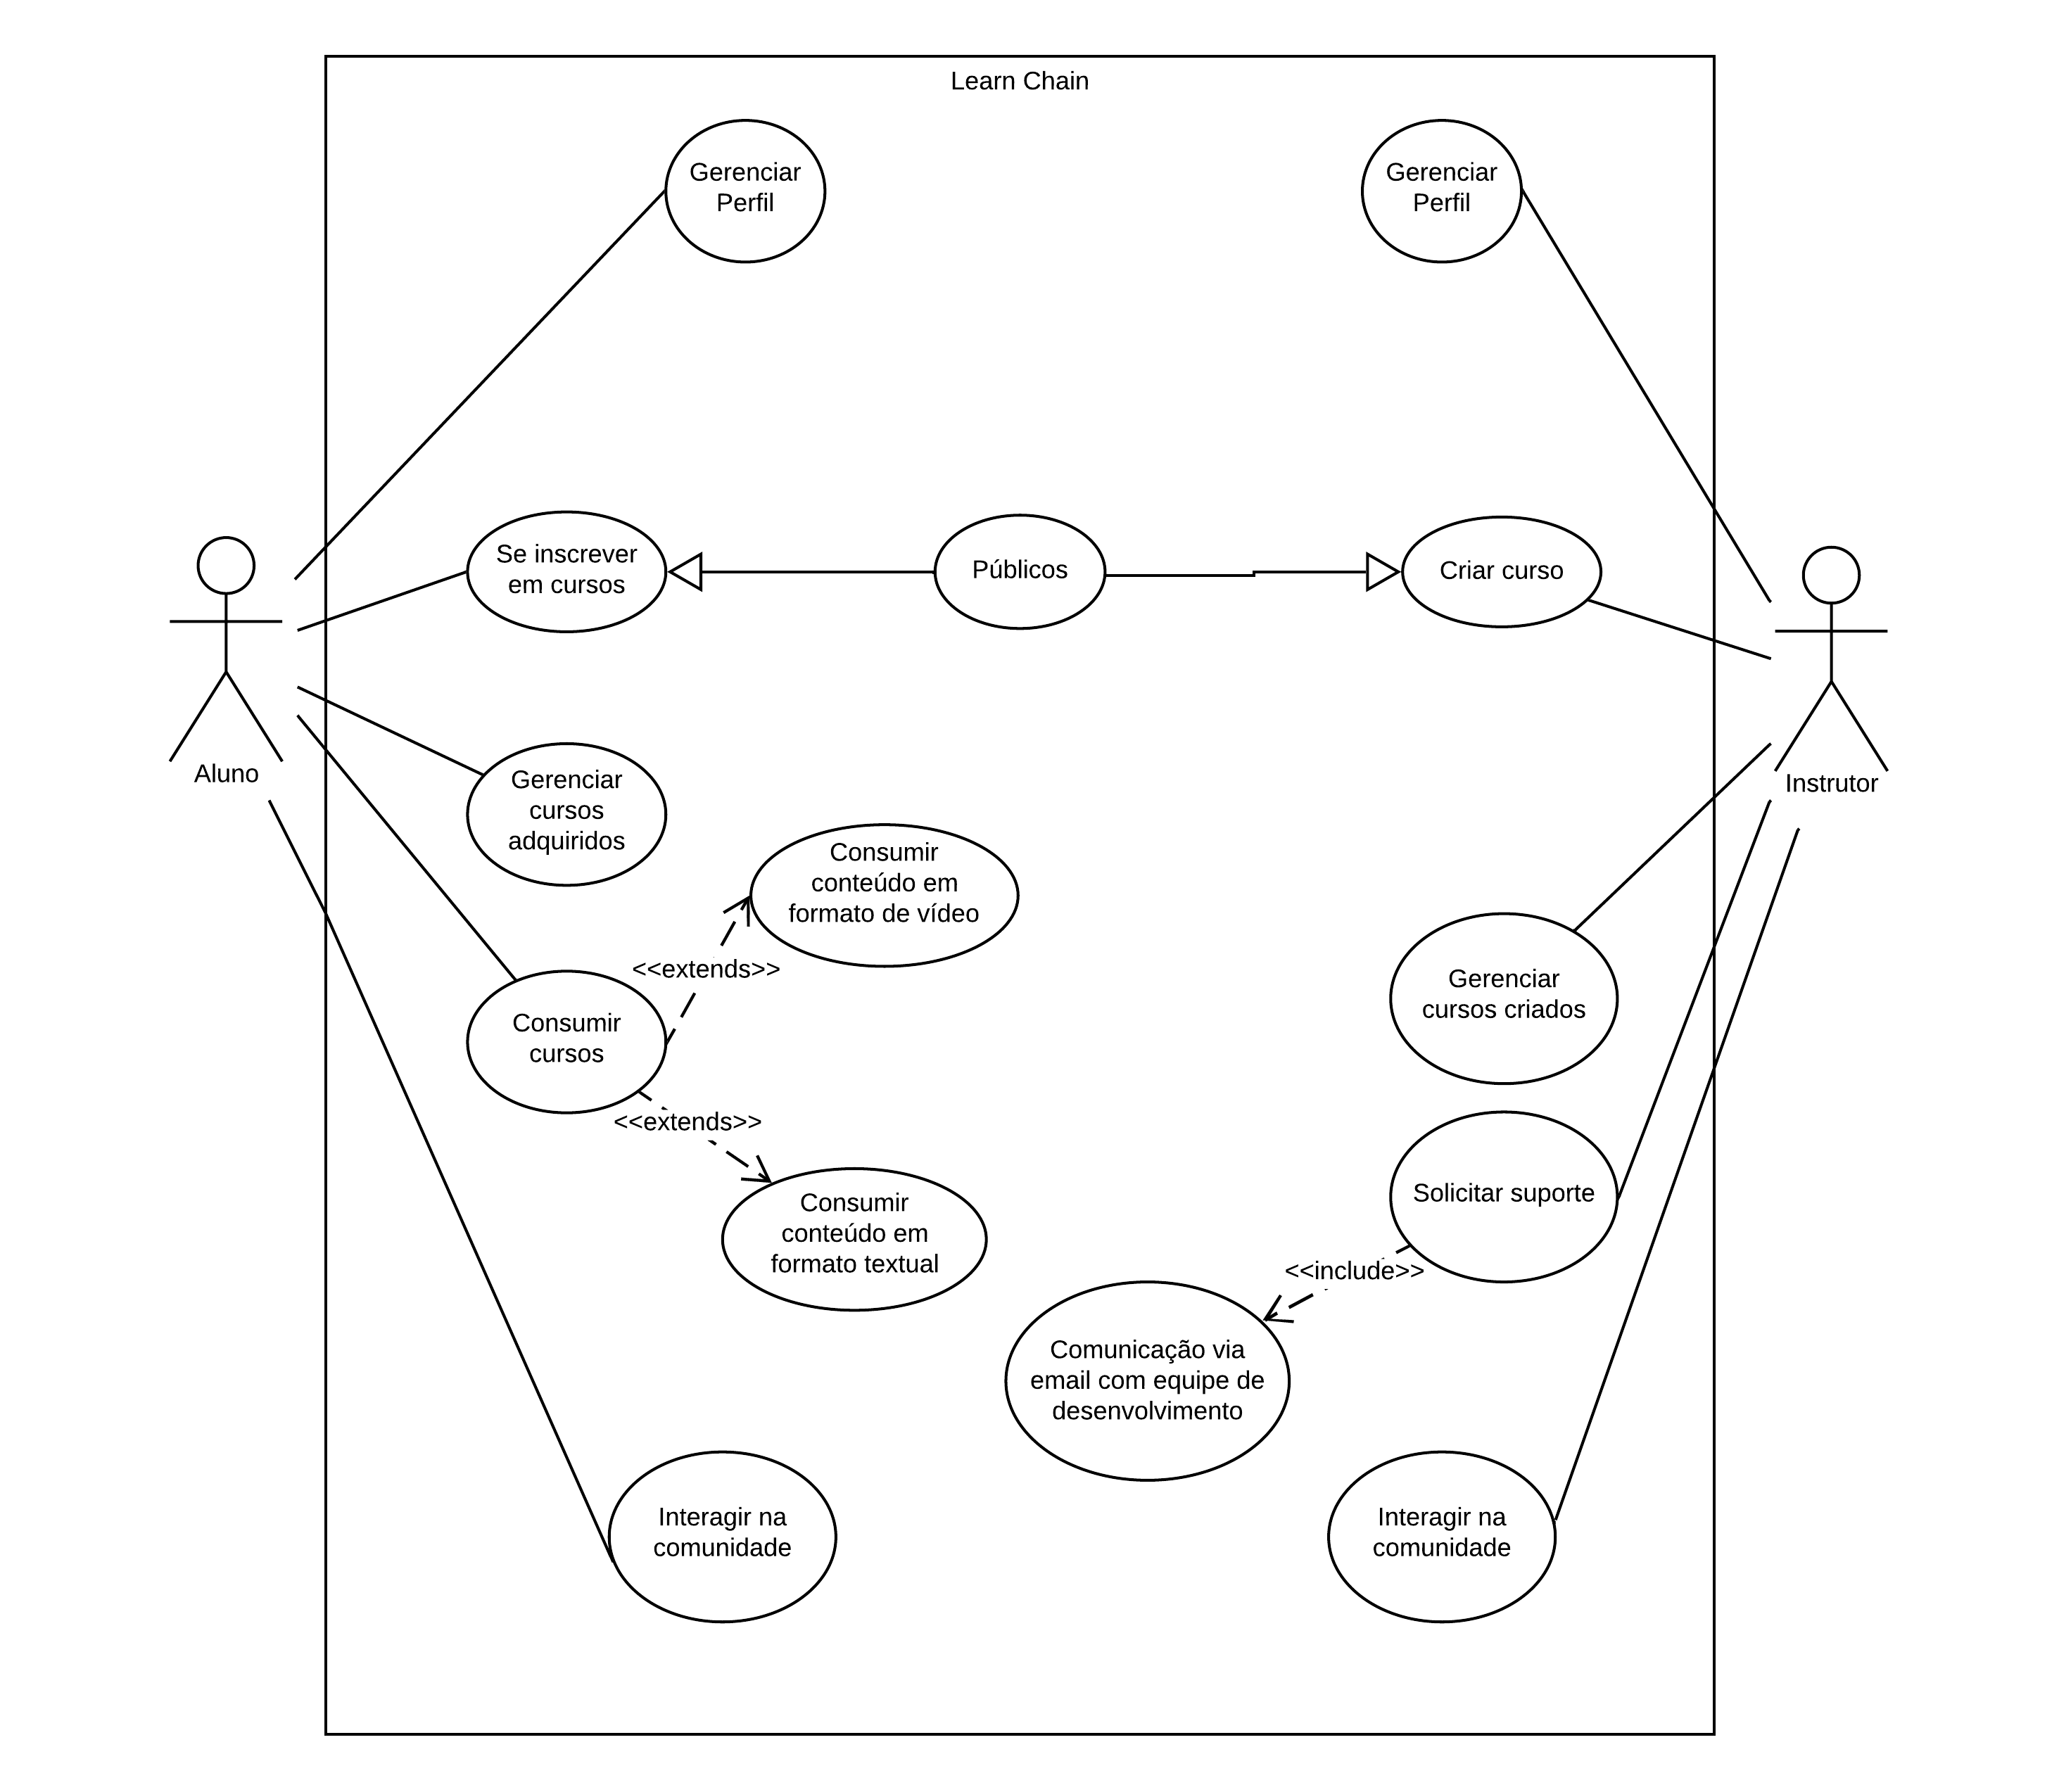
\includegraphics[width=0.8\textwidth]{figuras/uml.png}
            \begin{center}
                {\footnotesize Fonte: Autores}
            \end{center}
            \label{fig:diagrama}
        \end{figure}
        
        \subsubsection{Especificação dos casos de uso}

        Nesta seção, são apresentados os casos de uso levantados durante a elicitação dos requisitos do sistema e por meio de \textit{brainstorming}, estando sujeitos a alterações ao longo do desenvolvimento do projeto.

        \section*{UC01: Gerenciar Perfil}

        \begin{itemize}
            \item \textbf{Descrição:} Permite que um instrutor ou aluno cadastre, edite e exclua sua conta, além de realizar \textit{login} e \textit{logout}.
            
            \item \textbf{Ator Principal:} Instrutor e Aluno
            
            \item \textbf{Prioridade:} Alta
            
            \item \textbf{Pré-condição:} Usuário deve estar cadastrado na plataforma.
            
            \item \textbf{Fluxo Principal:}
            \begin{enumerate}
                \item Usuário se cadastra na plataforma.
                \item Sistema valida os dados e os salva.
                \item Usuário acessa a aba de gerenciamento de perfil.
                \item Usuário edita suas informações e clica em "Salvar".
                \item Usuário realiza \textit{logout}.
                \item Sistema encerra a sessão do usuário.
            \end{enumerate}

            \item \textbf{Fluxo Alternativo:}
            \begin{itemize}
                \item \textit{Dados Inválidos:}
                \begin{enumerate}
                    \item Caso os dados sejam inválidos, o sistema exibe uma mensagem de erro.
                    \item O sistema oferece a opção "Esqueci minha senha".
                    \item Usuário utiliza o /textit{e-mail} para recuperação de senha.
                    \item O sistema envia um /textit{e-mail} com instruções para redefinição de senha.
                \end{enumerate}
            \end{itemize}
        \end{itemize}

        \section*{UC02: Inscrever-se em Cursos}

        \begin{itemize}
            \item \textbf{Descrição:} Permite que um aluno se inscreva em cursos gratuitos disponíveis na plataforma.
            
            \item \textbf{Ator Principal:} Aluno
            
            \item \textbf{Prioridade:} Alta
            
            \item \textbf{Pré-condição:} Usuário deve estar cadastrado na plataforma.
            
            \item \textbf{Fluxo Principal:}
            \begin{enumerate}
                \item Aluno visualiza a lista de cursos disponíveis.
                \item Sistema exibe os cursos gratuitos disponíveis.
                \item Usuário se inscreve no curso desejado.
                \item Sistema registra a inscrição do usuário no curso.
            \end{enumerate}

            \item \textbf{Fluxo Alternativo:}
            \begin{itemize}
                \item \textit{Usuário já inscrito:}
                \begin{enumerate}
                    \item Aluno tenta se inscrever em um curso no qual já está matriculado.
                    \item Sistema exibe mensagem informando que o aluno já está registrado no curso.
                \end{enumerate}
            \end{itemize}
        \end{itemize}

        % \section*{UC03: Inscrever-se em Cursos Privados}

        % \begin{itemize}
        %     \item \textbf{Descrição:} Permite que um aluno se inscreva em cursos privados mediante pagamento.
            
        %     \item \textbf{Ator Principal:} Aluno
            
        %     \item \textbf{Prioridade:} Baixa
            
        %     \item \textbf{Pré-condição:} Usuário deve estar cadastrado na plataforma.
            
        %     \item \textbf{Fluxo Principal:}
        %     \begin{enumerate}
        %         \item Aluno visualiza a lista de cursos disponíveis.
        %         \item Sistema exibe os cursos privados disponíveis.
        %         \item Usuário se inscreve no curso desejado e realiza o pagamento.
        %         \item Sistema confirma o pagamento, registra a inscrição e disponibiliza o conteúdo.
        %     \end{enumerate}

        %     \item \textbf{Fluxo Alternativo:}
        %     \begin{itemize}
        %         \item \textit{Pagamento não realizado:}
        %         \begin{enumerate}
        %             \item Aluno tenta se inscrever sem concluir o pagamento.
        %             \item Sistema impede a inscrição até que o pagamento seja efetuado.
        %         \end{enumerate}
        %     \end{itemize}
        % \end{itemize}

        \section*{UC03: Gerenciar Cursos Adquiridos}

        \begin{itemize}
            \item \textbf{Descrição:} Permite que um aluno gerencie os cursos adquiridos e acompanhe seu progresso.
            
            \item \textbf{Ator Principal:} Aluno
            
            \item \textbf{Prioridade:} Alta
            
            \item \textbf{Pré-condição:} Usuário deve ter adquirido pelo menos um curso.
            
            \item \textbf{Fluxo Principal:}
            \begin{enumerate}
                \item Aluno acessa a seção "Meus Cursos".
                \item Sistema exibe a lista de cursos adquiridos e o progresso de cada um.
            \end{enumerate}

            \item \textbf{Fluxo Alternativo:}
            \begin{itemize}
                \item \textit{Nenhum curso adquirido:}
                \begin{enumerate}
                    \item Aluno acessa "Meus Cursos", mas não possui nenhum curso.
                    \item Sistema exibe mensagem informando que o usuário não possui cursos.
                \end{enumerate}
            \end{itemize}
        \end{itemize}

        \section*{UC04: Consumir Cursos}

        \begin{itemize}
            \item \textbf{Descrição:} Permite que um aluno consuma o conteúdo dos cursos adquiridos.
            
            \item \textbf{Ator Principal:} Aluno
            
            \item \textbf{Prioridade:} Alta
            
            \item \textbf{Pré-condição:} Usuário deve ter adquirido pelo menos um curso.
            
            \item \textbf{Fluxo Principal:}
            \begin{enumerate}
                \item Aluno acessa a seção "Meus Cursos".
                \item Sistema exibe os cursos adquiridos e o progresso.
                \item Aluno seleciona um curso.
                \item Sistema exibe o conteúdo do curso (vídeo ou texto).
                \item Aluno consome o conteúdo.
            \end{enumerate}
        \end{itemize}

        \section*{UC05: Criar Cursos}

        \begin{itemize}
            \item \textbf{Descrição:} Permite que um instrutor crie novos cursos na plataforma.
            
            \item \textbf{Ator Principal:} Instrutor
            
            \item \textbf{Prioridade:} Alta
            
            \item \textbf{Pré-condição:} Instrutor deve estar cadastrado.
            
            \item \textbf{Fluxo Principal:}
            \begin{enumerate}
                \item Instrutor acessa a opção "Criar Curso".
                \item Sistema exibe os campos necessários para criação do curso.
                \item Instrutor preenche os campos obrigatórios.
                \item Sistema permite o \textit{upload} de vídeos e textos.
                \item Instrutor adiciona conteúdos conforme necessário.
                \item Sistema salva o curso criado.
            \end{enumerate}

            \item \textbf{Fluxo Alternativo:}
            \begin{itemize}
                \item \textit{Campos obrigatórios não preenchidos:}
                \begin{enumerate}
                    \item Instrutor tenta criar o curso sem preencher os campos obrigatórios.
                    \item Sistema impede a criação e exibe mensagem de erro.
                \end{enumerate}
            \end{itemize}
        \end{itemize}

        \section*{UC06: Gerenciar Cursos Criados}

        \begin{itemize}
            \item \textbf{Descrição:} Permite que um instrutor gerencie os cursos criados, podendo editá-los ou removê-los.
            
            \item \textbf{Ator Principal:} Instrutor
            
            \item \textbf{Prioridade:} Média
            
            \item \textbf{Pré-condição:} Instrutor deve ter criado pelo menos um curso.
            
            \item \textbf{Fluxo Principal:}
            \begin{enumerate}
                \item Instrutor acessa a seção "Meus Cursos Criados".
                \item Sistema exibe os cursos criados pelo instrutor.
                \item Instrutor pode editar ou excluir cursos conforme necessário.
                \item Sistema salva as alterações realizadas.
            \end{enumerate}

            \item \textbf{Fluxo Alternativo:}
            \begin{itemize}
                \item \textit{Nenhum curso criado:}
                \begin{enumerate}
                    \item Instrutor acessa a seção "Meus Cursos Criados", mas não possui cursos.
                    \item Sistema exibe mensagem informando que o instrutor não possui cursos.
                \end{enumerate}
            \end{itemize}
        \end{itemize}

        \section*{UC07: Instrutor solicitar suporte}

        \begin{itemize}
            \item \textbf{Descrição:} Permite que o instrutor solicite ajuda quanto ao uso da plataforma ou algum problema.
            
            \item \textbf{Ator Principal:} Instrutor
            
            \item \textbf{Prioridade:} Alta
            
            \item \textbf{Pré-condição:} Instrutor deve ter efetuado cadastro na plataforma.
            
            \item \textbf{Fluxo Principal:}
            \begin{enumerate}
                \item Instrutor acessa a seção "Ajuda".
                \item Sistema disponibiliza área de comentários para instrutor enviar mensagem.
                \item Instrutor escreve mensagem e clica em enviar.
                \item Sistema recebe notificação e notifica a equipe de desenvolvimento.
                \item Equipe trata da situação via /textit{email} com instrutor.
            \end{enumerate}
        \end{itemize}

        \section*{UC08 Aluno interagir na comunidade}

        \begin{itemize}
            \item \textbf{Descrição:} Permite que aluno interaja na comunidade, expressando-se com outros usuários a respeito do conteúdo do curso.
            
            \item \textbf{Ator Principal:} Alunos.
            
            \item \textbf{Prioridade:} Baixa
            
            \item \textbf{Pré-condição:} Usuário deve possuir um curso.
            
            \item \textbf{Fluxo Principal:}
            \begin{enumerate}
                \item Usuário acessa sessão de comunidade.
                \item Sistema disponibiliza área para escrita.
                \item Usuário escreve alguma dúvida, observação ou informação pertinente.
                \item Sistema salva comentário e notifica instrutor.
            \end{enumerate}
        \end{itemize}

        \section*{UC09: Instrutor interagir na comunidade}

        \begin{itemize}
            \item \textbf{Descrição:} Permite que instrutor interaja na comunidade, ajudando os alunos do curso.
            
            \item \textbf{Ator Principal:} Instrutor.
            
            \item \textbf{Prioridade:} Baixa
            
            \item \textbf{Pré-condição:} Instrutor deve ter criado um curso.
            
            \item \textbf{Fluxo Principal:}
            \begin{enumerate}
                \item Instrutor acessa sessão de comunidade.
                \item Sistema disponibiliza os comentários realizados pelos alunos.
                \item Intrutor interaje com os alunos.
                \item Sistema salva comentário e notifica alunos.
            \end{enumerate}
        \end{itemize}


        \subsubsection{Prototipação}

        O processo de prototipação é fundamental para o sucesso de um software, pois é por ele que é possível validar o design, a usabilidade e a experiência do usuário antes da implementação inicial. Neste projeto, o protótipo de alta fidelidade foi dividido em duas (2) etapas: elaboração do guia de estilo, contento cores, espaços e tipografia, e desenvolvimento das telas da interface propriamente dita. 

        A Figura \ref{fig:guia-de-estilo} representa o guia de estilo do projeto, enquanto as figuras \ref{fig:Registro}, \ref{fig:main}, \ref{fig:detalhamento_do_curso}, \ref{fig:Criar_conteudo_didatico}, \ref{fig:meus_cursos}, \ref{fig:Criando_curso} são referentes as telas do sistema.

\section{Arquitetura do Software}
A construção de uma aplicação percorre várias etapas, desde a concepção da ideia e validação até a prototipação e, seguidamente, codificação resultando em uma solução. Para atingir esse objetivo de maneira eficiente, é necessário escolher ferramentas e tecnologias que suportem  o tamanho e robustez que a aplicação se propõe. No projeto Learn Chain, serão utilizadas tecnologias que atendam esses critérios.

A arquitetura proposta segue o modelo Cliente-Servidor com adaptação para uso da rede distribuída IPFS. Essa arquitetura visa utilizar as vantagens do cliente-servidor para gerenciamento dos clientes da aplicação e referência das chaves únicas do conteúdo dos cursos que serão persistidos no sistema distribuído, fazendo assim com que o ponto chave desse projeto, que são os cursos, fiquem acessíveis nesta rede.

A Figura \ref{fig:arquitetura_sistema} apresenta a arquitetura do sistema projetada para o desenvolvimento da aplicação. Essa arquitetura foi concebida para garantir escalabilidade, segurança e descentralização, alinhando-se aos requisitos definidos na proposta.

\begin{figure}[h]
    \centering
    \caption{Arquitetura do sistema.}
    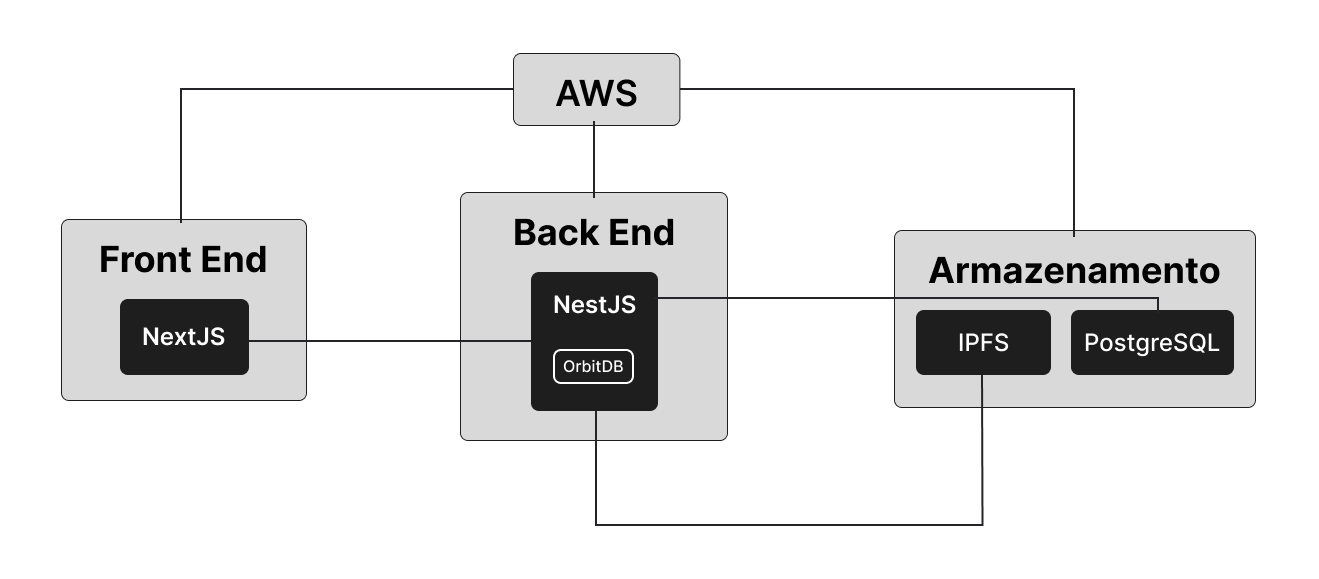
\includegraphics[width=0.8\textwidth]{figuras/arquitetura.png}
    \begin{center}
        {\footnotesize Fonte: Autores}
    \end{center}
    \label{fig:arquitetura_sistema}
\end{figure}

\subsection{Arquitetura de desenvolvimento web}

A arquitetura cliente-servidor será adotada no desenvolvimento da aplicação, devido à sua robustez e flexibilidade no gerenciamento de interações entre usuários e servidores. Nesse modelo, os clientes fazem requisições a um servidor centralizado, que processa as solicitações e retorna as respostas adequadas. A utilização dessa abordagem oferece uma série de benefícios importantes para o desenvolvimento do sistema. A seguir, estão algumas vantagens deste modelo arquitetural.

\subsection{Principais vantagens do modelo Cliente-Servidor}

De acordo com Coulouris et al. (2011)\cite{coulouris2011}, o modelo cliente-servidor apresenta diversas vantagens que o tornam uma escolha recorrente em sistemas distribuídos, especialmente quando se deseja equilibrar controle, desempenho e escalabilidade.

\begin{itemize}
    \item \textbf{Controle:} Apesar do cerne desta aplicação ser a descentralização e democratização dos dados, a gestão dos usuários foi pensada de forma centralizada. Esse modelo permite maior integridade e consistência das informações, reduzindo riscos de dados corrompidos ou acessos indevidos.
    
    \item \textbf{Escalabilidade:} A arquitetura cliente-servidor é capaz de comportar um número elevado de usuários, com possibilidade de aprimoramento conforme a demanda aumenta.
    
    \item \textbf{Desempenho e Eficiência:} A separação entre cliente e servidor otimiza o desempenho da aplicação, permitindo que o cliente se concentre na interação com o usuário e o servidor se encarregue do processamento e armazenamento de dados.
    
    \item \textbf{Facilidade de Manutenção e Atualização:} Como o processamento está centralizado no servidor, as atualizações e manutenções podem ser realizadas em um único ponto, simplificando a implantação de melhorias e correções.
    
    \item \textbf{Flexibilidade e Compatibilidade:} A arquitetura permite a distribuição da aplicação em diferentes plataformas, como web, desktop e dispositivos móveis, ampliando seu alcance e acessibilidade.
\end{itemize}

\section{Tecnologias da aplicação}

\subsection{O \textit{InterPlanetary File System} (IPFS)}
\label{sec:ipfs}
O IPFS é um protocolo distribuído para armazenamento e compartilhamento de dados, que organiza arquivos em uma estrutura baseada em conteúdo, tornando a web mais eficiente e resistente a falhas \cite{ipfs2025}. Com ele é possível persistir os dados da aplicação entre os nós da rede. Isso o torna acessível, de fato, e replicável por quaisquer usuários que o quiserem. Diferente do HTTP, que carrega arquivos de um servidor, o IPFS utiliza um modelo de endereçamento de conteúdo, em que os dados são desacoplados de sua localização e tratados a partir da \textit{hash} única gerada pelo conteúdo do mesmo.

Entre suas principais características, destacam-se:

\begin{itemize}
    \item \textbf{Identificadores de Conteúdo (CIDs - \textit{Content Identifiers})}: cada conteúdo ou arquivo é associado a um endereço único baseado em um \textit{hash} criptográfico, garantindo sua integridade e imutabilidade.
    
    \item \textbf{Rede \textit{Peer-to-Peer} (P2P)}: milhares de nós interconectados facilitam a localização e recuperação dos dados distribuídos na rede.
    
    \item \textbf{Armazenamento em \textit{Cache}}: os dados são armazenados temporariamente na memória \textit{cache} dos nós, otimizando a largura de banda e melhorando a eficiência na redistribuição de conteúdos.
\end{itemize}

\subsubsection{Justificativa da escolha da tecnologia}
Neste projeto, o foco é desenvolver uma plataforma descentralizada para cursos e materiais educativos utilizando o IPFS para garantir que os dados permaneçam sob o controle direto de seus criadores. Ele será utilizado para o armazenamento descentralizado de conteúdos de aprendizagem, permitindo que os dados sejam acessados de maneira eficiente, sem depender de um único servidor. Através da identificação utilizando \textit{hashs} únicas, o IPFS garante a integridade do conteúdo, evitando duplicação desnecessária de arquivos na rede, além de tornar o sistema resistente a falhas e censura, uma vez que os dados podem ser distribuídos entre múltiplos nós na rede. A rede IPFS armazenará os dados dos cursos, tanto os públicos quanto os privados. Dessa forma, mesmo que eventualmente essa aplicação saia de circulação ou seja bloqueada, os dados permanecerão disponíveis globalmente ao público. O uso desta tecnologia elimina a dependência de servidores centrais, garantindo que seja alcançado o objetivo central deste projeto.

\subsection{OrbitDB: Banco de Dados Distribuído}

O OrbitDB é um banco de dados \textit{serverless} e ponto a ponto (\textit{peer-to-peer}) distribuído. Construído para atuar em aplicações descentralizadas, ele utiliza o IPFS para o armazenamento e sincronia dos dados entre os diferentes nós. Ele será utilizado no projeto para realizar a comunicação e persistência dos dados com a rede IPFS.

\subsubsection*{Pontos Fortes do OrbitDB:}
\begin{itemize}
    \item \textbf{Descentralização}: Dispensa a necessidade de servidores centralizados.
    \item \textbf{Alta disponibilidade}: Suporta replicação automática e sincronização entre nós.
    \item \textbf{Desempenho escalável}: Ideal para aplicações distribuídas que requerem persistência de dados em tempo real.
    \item \textbf{Fácil integração}: Compatível com tecnologias baseadas em JavaScript.
\end{itemize}

\subsubsection{Justificativa da escolha da tecnologia}
Ele foi escolhido por ser escrito em JavaScript, sendo possível a integração com a NestJS, tecnologia que será utilizada no desenvolvimento do \textit{backend}, além de facilitar a manipulação dos dados na rede IPFS.

\subsection{NestJS}

NestJS é uma \textit{framework} para construir aplicativos Node.js eficientes e escaláveis. Ele utiliza JavaScript progressivo, sendo construído com e oferecendo suporte total a TypeScript (mas ainda permitindo que os desenvolvedores codifiquem em JavaScript puro). Ele combina elementos de POO (Programação Orientada a Objetos), FP (Programação Funcional) e FRP (Programação Reativa Funcional) \cite{nestjs2025}.

\subsubsection*{Pontos Fortes do NestJS:}
\begin{itemize}
    \item \textbf{Modularidade}: Arquitetura que facilita a divisão da aplicação em módulos reutilizáveis.
    \item \textbf{Integração simples com bancos de dados}: Compatível com ORM populares, como TypeORM e Prisma.
    \item \textbf{Injeção de Dependência}: Simplifica o gerenciamento de dependências e aumenta a testabilidade.
    \item \textbf{Flexibilidade}: Suporta diversos paradigmas, como programação reativa e microsserviços.
\end{itemize}

\subsubsection{Justificativa da escolha da tecnologia}
NestJS foi escolhido para a estrutura do \textit{backend} da aplicação por sua compatibilidade com JavaScript e TypeScript, além de sua arquitetura modular e suporte a injeção de dependências. Sua integração nativa com o OrbitDB permite uma comunicação eficiente com o banco de dados distribuído, enquanto seu suporte ao PostgreSQL garante um armazenamento seguro e estruturado para os dados dos usuários.

\subsection{Next.js}

O \textbf{Next.js} é um \textit{framework} React para desenvolvimento de aplicações no lado do cliente. Ele oferece recursos como renderização no lado do servidor (\textit{Server-Side Rendering} - SSR) e geração de \textit{sites} estáticos (\textit{Static Site Generation} - SSG), que permitem criar interfaces modernas com excelente desempenho.

\subsubsection*{Pontos Fortes do Next.js:}
\begin{itemize}
    \item \textbf{Renderização otimizada}: Suporte a SSR e SSG, melhorando o desempenho e SEO.
    \item \textbf{Rotas automáticas}: Simplifica a estrutura de navegação com rotas baseadas em arquivos.
    \item \textbf{Desenvolvimento eficiente}: \textit{Hot reloading} e compilação automática durante o desenvolvimento.
    \item \textbf{\textit{API Routes}}: Permite criar APIs no mesmo projeto do \textit{front-end}.
    \item \textbf{Suporte ativo da comunidade}: Grande número de extensões e soluções prontas.
\end{itemize}

\subsubsection{Justificativa da escolha da tecnologia}
No contexto deste trabalho, o Next.js foi escolhido para desenvolver a interface da aplicação, garantindo carregamento eficiente e uma experiência fluida para os usuários. Além disso, o Next.js traz recursos como otimização automática de imagens, roteamento intuitivo e suporte integrado a APIs, facilitando a implementação de uma interface interativa e responsiva para o projeto \cite{nextjs2025}. 

\subsection{PostgreSQL}

O \textbf{PostgreSQL} é um Sistema de Gerenciamento de Banco de Dados (SGBD) muito utilizado no desenvolvimento web, sendo conhecido por sua flexibilidade e desempenho. É um dos sistemas de armazenamento de dados mais seguros e confiáveis da atualidade, promovendo segurança e integridade dos dados, principalmente por sua conformidade com os princípios ACID (Atomicidade, Consistência, Isolamento e Durabilidade). 

\subsubsection*{Pontos Fortes do PostgreSQL:}
\begin{itemize}
    \item \textbf{Suporte Avançado a Dados}: Compatível com tipos complexos, como JSON, \textit{arrays}, e dados geoespaciais (\textit{PostGIS}).
    \item \textbf{Alta Conformidade com Padrões SQL}: Facilita a portabilidade de aplicações entre diferentes bancos de dados.
    \item \textbf{Extensibilidade}: Suporte a funções definidas pelo usuário, tipos de dados customizados e linguagens de programação adicionais.
    \item \textbf{Desempenho e Escalabilidade}: Otimizações para consultas complexas e grandes volumes de dados, com suporte a replicação e particionamento.
    \item \textbf{Segurança}: Autenticação robusta, criptografia e controle granular de permissões.
    \item \textbf{Comunidade Ativa}: Grande quantidade de documentação e suporte da comunidade global.
\end{itemize}

\subsubsection{Justificativa da escolha da tecnologia}
O PostgreSQL está sendo utilizado para armazenar os usuários da plataforma, e também dos metadados dos materiais de cursos da plataforma. Além das características de confiabilidade, sua escolha também foi influenciada pela experiência dos membros desenvolvedores com tal tecnologia. Outro aspecto relevante para a escolha do PostgreSQL é sua compatibilidade com diferentes arquiteturas computacionais, incluindo os sistemas distribuídos. Ele é uma ótima opção para lidar com otimicações de indexação, que garante maior eficiência na busca por informações, oferecendo melhor experiência aos usuários utilizadores do sistema por uma vantagem no tempo de carregamento. Por fim, a experiência prévia da equipe de desenvolvimento com essa tecnologia também influenciou a decisão, assegurando maior agilidade e segurança na implementação do banco de dados.

\subsubsection{Diagrama lógico de dados}
O diagrama lógico de dados (DLD) se propõe a ser um modelo de dados de um sistema a partir de tabelas, colunas, dados e relacionamentos a fim de facilitar a implementação no banco PostgreSQL \cite{lucidchart2025}.

A Figura \ref{fig:dld} apresenta o Diagrama Lógico de Dados (DLD) proposto para a solução Learn Chain, detalhando os relacionamentos entre as tabelas e os atributos de cada uma. Vale ressaltar que este diagrama não inclui a modelagem que estará presente na rede IPFS, pois todos os dados serão armazenados no formato JSON. A interface entre os dados armazenados no IPFS e o banco de dados é realizada por meio da tabela ContentIPFSRef, a qual armazena o CID, um \textit{hash} que serve como chave de acesso aos dados no IPFS. Essa estrutura permite a comunicação eficiente entre o banco de dados e a rede descentralizada, conforme discutido na subseção \ref{sec:ipfs}.

\section{Ferramentas de suporte técnico}
Para o auxílio durante o desenvolvimento do presente trabalho, estão sendo utilizadas as ferramentas:

\begin{itemize}
    \item \textbf{Discord}: Plataforma de comunicação com canais de texto e voz. Utilizada principalmente para comunicação síncrona entre os desenvolvedores, sendo fundamental para realizar a prática de \textit{pair programming}.
    \item \textbf{Git e GitHub}: Git é uma tecnologia de controle de versões de artefatos, e GitHub é a hospedagem de repositórios. Utilizados para gerenciar as versões do documento escrito.
    \item \textbf{Trello}: Ferramenta de gerenciamento de projetos baseada em Kanban. Utilizado para organizar tarefas e acompanhar o progresso do projeto.
    \item \textbf{LaTeX}: É uma linguagem de marcação uilizada para a formatação de documentos. Ela foi utilizada para a criação de toda a redação deste trabalho.
    \item \textbf{Visual Studio Code}: Editor de código-fonte gratuito, multiplataforma e personalizável. Desenvolvido pela Microsoft, está sendo utilizado como suporte para interpretação da linguagem LaTeX.
    \item \textbf{Lucidchart}: É uma ferramenta \textit{online} que permite criar diagramas, fluxogramas, \textit{wireframes} e mapas de processos. Tal tecnologia está sendo utilizada para a construção de diagramas de casos de uso.
    \item \textbf{Figma}: Tipo de ferramenta do design gratuita que permite criar protótipos e interfaces de aplicações. Está sendo utilizada para desenvolver o protótipo.
    \item \textbf{Dbdiagram}: É uma ferramenta de criação de diagramas e scripts de banco de dados. Foi utilizada para a construção do DLD.
    \item \textbf{Google Meet}: Plataforma de videoconferência desenvolvida pelo Google. Foi utilizada para a realização do \textit{brainstorming}.
\end{itemize}